\chapter{NMT-Basierte Modelle}

In den zwei vorangegangenen Kapiteln wurde die Struktur von BERT \ref{BERT} und Transformer \ref{transformer} vorgestellt. Das Kapitel 6 beschäftigt sich mit Neural-Machine-Translation-Modellen (NMT), mit denen versucht wurde, Sätze in einfache Sprache zu übersetzen. Die Struktur der Modelle wird zuerst dargestellt und anschließend wird die Vorführung gegeben, wie diese Modelle in Python eingesetzt werden können. Zum Schluss werden die Erkenntnisse für jedes Modell zusammengefasst.

\section{BERT Neural Machine Translation Model}
In \cite{NMT:20} wird ein Modell vorgestellt, das auf dem üblichen Transformer basiert und im wessen Kern BERT und Neural Machine Translation (NMT) Model zusammenarbeiten. Das NMT-Model ist der bekannte Transformer (siehe \cref{Transformer}). Im oben genannten Artikel wird das in dieser Arbeit verwendete Modell als BERT-fused Model beschrieben, jedoch wird es für die vorliegenden Zwecke BERT-Neural-Machine-Translation Modell, oder BNMT, genannt.

\subsection{Struktur des BNMT-Model}\label{sec:BNMT_Model}
Die Struktur des Modells ist durch die folgende \cref{bnmt_model_figure} gegeben.

Die Autoren des Artikels \cite{NMT:2017} schlagen vor, dass die Eingabe vorerst in ein BERT-Modell fließt, dessen Ausgabe später in den Encoder und Decoder des Transformer-Models verläuft. Der Flussverlauf von Informationen wird im \cite{NMT:20} in drei Schritte aufgeteilt.

\begin{figure}[H]
	\centering
	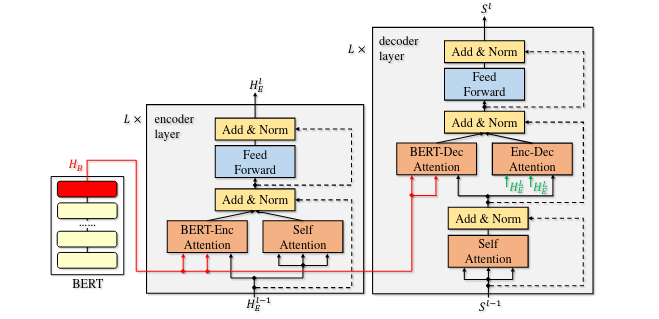
\includegraphics[scale=0.7]{images/BNMT-Model.png}
	\caption{BNMT-Model Struktur \cite{NMT:20}}
	\label{bnmt_model_figure}
\end{figure}

Vorerst werden einige Notationen eingeführt. Die Datensätze für die Eingabe- sowie Targetsätze werden durch \textit{X} bzw. durch \textit{Y} markiert. Für jeden beliebigen Satz \textit{x} $\in$ \textit{X} und \textit{y} $\in$ \textit{Y} bezeichnet $l_x$ und $l_y$ die Anzahl der Wörter in diesen Einträgen. Die einzelnen Elemente in \textit{x} oder \textit{y} werden entsprechend ihrer Position mit $x_i$ bzw. $y_i$ gekennzeichnet.

\begin{enumerate}
	\item Schritt 1: Bei einer Eingabe \textit{x} $\in$ \textit{X}, wo \textit{X} die Menge der Eingaben ist, bettet BERT den \textit{x}-Vektor als $H_B = BERT(x)$ ein, wobei $H_B$ die Ausgabe des letzten Layers vom BERT ist, während $h_{B,i} \in H_B$ das \textit{i}-te Element der Ausgabe darstellt. \label{step_1_text}
	
	\item Schritt 2: Die Variable $H^l_E$ wird genutzt, um die Darstellung der versteckten \textit{l}-ten Schicht zu beschreiben, wobei $H^0_E$ die Einbettung der Sequenz \textit{x} ist. Das \textit{i}-te Element aus $H^l_E$ wird als $h^l_i$ für $0<i<[l_x]$ definiert (begrenzt durch die Anzahl der Neuronen in jeder versteckten Schicht \textit{l}). Die Berechnung von $h^l_i$ ist wie folgt gegeben, dabei sind $attn_S$ und $attn_B$ die Attention-Modelle bzw. MHA-Schichten mit unterschiedlichen Parametern (die Definition ist in \cref{MHA_Layer} zu finden): \label{step_2_text}
	
	\begin{equation}\label{step_2}
		\tilde{h}^l_i = \frac{1}{2}(attn_S(h^{l-1}_i, H^{l-1}_E, H^{l-1}) + attn_B(h^{l-1}_i, H_B, H_B)), \text{ für } 0 < i < [l_x]
	\end{equation}
	
	Weiterhin werden die berechneten Attentions $\tilde{h}^l_i$ nach ihrer Normierung dem Feed-Forward-Network eingeflossen und schließlich wird die Ausgabe standardisiert. Die Ausgabe aus der letzten Schicht ist durch $H^L_E$ definiert.	
	
	\item Schritt 3: Die Eingabe im Decoder-Layer \textit{l} wird durch $S^l_{<t}$ für den Zeitpunkt \textit{t}, $S^l_{<t} = (s^l_1, · · · , s^l_{t−1})$ bezeichnet. $s^0_1$ ist ein besonderes Zeichen, das den Anfang der Sequenz bestimmt und $s^0_t$ ist die Voraussage des Modells zum bestimmten Zeitpunkt \textit{t}. In der Schicht \textit{l} erfolgt Folgendes: 	
	\begin{subequations}
		\label{step_3}
		\begin{gather}
			s^lt = attn_S (s^{l−1}t , S^{l−1}_{<t+1}, S^{l−1}_{<t+1})\\
			\~s^l_t = 1/2(attn_B (\ˆs^l_t, H_B , H_B ) + attn_E (\ˆs^l_t, H^L_E, H^L_E )), \text{ } s^l_t = FFN( ̃s^l_t)
		\end{gather}
	\end{subequations}\label{step_3_text}
\end{enumerate}


Die $attn_S$, $attn_B$ und $attn_E$ stellen entsprechend Self-, BERT-Decoder- und Encoder-Decoder-Attention dar. Die \cref{step_3} führt eine Iteration über die Schichten und liefert das Ergebnis $s^L_t$. Die Ausgabe fließt durch eine Dense-Schicht und wird schließlich von einer Softmax-Funktion transformiert, was dazu führt, dass das \textit{t}-te Wort $\^y_t$ prognostiziert werden kann. Diese Schritte iterieren, bis ein Endzeichen erreicht wird, bzw. bis das Ende der Sequenz verarbeitet wird.

\subsection{Implementierung}

Als Nächstes wird ein Modell vorgestellt. Das Modell verwendet BERT für die Einbettung zu Beginn des Prozesses. Für die Implementierung werden die Bibliotheken \textit{tensorflow} und \textit{transformers} benutzt.

Das Modell wird in einige Elemente aufgeteilt. Manche Komponenten werden von der Tensorflow-Bibliothek bereitgestellt. Die Klasse des Modells ist gegeben:

\begin{lstlisting}[language=Python, caption={BNMT\_Model}, label={lis:BNMT_Model}]
	# 1. Layer (BERT-Model)
	self.bert_layer = transformers.TFBertModel.from_pretrained(model_name)
	# 2. Layer Encoder Embedding layer
	self.enc_embedding_layer = Embedding(vocab_size, hidden_layer_size, input_length=seq_len)
	# 3. Layer Encoder
	self.encoder_layers = [NMTEncoderLayer(hidden_layer_size, transformer_heads, 1e-3) for _ in range(transformer_heads)]
	# 4. Decoder Embedding
	self.decoder_emb = Embedding(vocab_size, hidden_layer_size, input_length=seq_len)
	# 5. Layer (Decoder)
	self.decoder_layers = [NMTDecoderLayer(hidden_layer_size, transformer_heads, 1e-3) for _ in range(transformer_heads)]
	# 6. Layer (Translation layer) 
	self.dense_layer = tf.keras.layers.Dense(vocab_size)
	self.softmax_layer = tf.keras.layers.Softmax()
\end{lstlisting}

Somit darf das Modell in sechs größere Komponenten zerlegt werden. Die erste Komponente erledigt die BERT-Einbettung. Zu diesem Zweck wird ein vortrainiertes BERT-Modell verwendet, das explizit an die deutsche Sprache angepasst ist. Das Modell ist von den Entwicklern von deepset.ai \cite{bert_based:19} bereitgestellt worden. Es ist ein standard BERT-Base Modell (\cref{lis:BERT_Base}). Zeilen 4 bis 10 im \cref{lis:BNMT_Model} beschreiben die Encoder- und Decoder-Modelle. Die letzten zwei Zeilen (12 und 13) beschreiben die Inferenz des Modells (Übersetzungsschicht). Die Ausgabe vom Decoder wird durch die Dense-Schicht erweitert, sodass sie die vorliegende Datensammlung repräsentiert. Als letztes wird eine Softmax-Funktion angewendet und als Ergebnis wird die Wahrscheinlichkeit für jedes Wort aus der Datensammlung, in der Sequenz vorzukommen, berechnet. 

Die Encoder und Decoder im NMT-Modell sind modifiziert, um die Vorteile des vortrainierten BERT-Modells zu nutzen. Nach der \cref{bnmt_model_figure} und den Formeln aus \cref{sec:BNMT_Model} werden die beiden Schichten wie folgt eingesetzt:

\begin{itemize}
	\item Der Encoder: 
	\begin{lstlisting}[language=Python, caption={BNMT\_Encoder}, label={BNMT_Encoder_init}]
		self.self_mha = NMTMultiHeadAttention(d_model, num_heads)
		self.bert_mha = NMTMultiHeadAttention(d_model, num_heads)
		
		self.ffn = self.point_wise_feed_forward_network(d_model, dff)
		
		self.normalization_Layer = LayerNormalization(epsilon=1e6)
		self.normalization_Layer2 = LayerNormalization(epsilon=1e6)	
		
		self.drop_layer1 = Dropout(drop_rate)
		self.drop_layer2 = Dropout(drop_rate)
	\end{lstlisting}
	In den Zeilen 1 und 2 werden die zwei Attention-Schichten initialisiert. Die erste und zweite Normierungsschicht werden in Zeilen 6 und 7 erstellt. Die letzte Komponente im Encoder wird in der Zeile 4 durch die Methode \\ \textit{point\_wise\_feed\_forward\_network} geliefert. Zwei zusätzliche Dropout-Layers werden instanziiert.
	\item Der Decoder:	
	\begin{lstlisting}[language=Python, caption={BNMT\_Decoder}, label={BNMT\_Decoder}]
		self.self_mha = NMTMultiHeadAttention(d_model, num_heads)
		self.bert_dec_mha = NMTMultiHeadAttention(d_model, num_heads)
		self.enc_dec_mha = NMTMultiHeadAttention(d_model, num_heads)
		
		self.ffn = self.point_wise_feed_forward_network(d_model, dff)
		
		self.norm_layer = LayerNormalization(epsilon=1e-6)
		self.norm_layer2 = LayerNormalization(epsilon=1e-6)
		self.norm_layer3 = LayerNormalization(epsilon=1e-6)
		
		self.drop_layer1 = Dropout(drop_rate)
		self.drop_layer2 = Dropout(drop_rate)
		self.drop_layer3 = Dropout(drop_rate)
	\end{lstlisting}
\end{itemize}
	Im Decoder werden drei Attention-Layers nach \cref{fig:NMT_Model}, die in Zeilen 1 bis 3 erstellt werden, angewendet. Jedem Multi-Head-Attention-Layer folgt eine Normierungsschicht. Die Schichten sind in den Reihen 7 bis initialisiert. Für die Erstellung des Feed-Forward-Network wird die gleiche Methode wie im Encoder verwendet. Im Decoder werden drei Dropout-Schichten eingesetzt, eine nach jedem Schritt.

%Schließlich ergibt sich folgende Ausführungsmethode:
%
%\begin{lstlisting}[language=Python, caption={BNMT\_call}]
%	inp, target = inputs
%	enc_padding_mask, dec_padding_mask, look_ahead_mask = self.create_masks(inp['input_ids'], target)
%	
%	# Embedding (Step 1.)
%	enc_out = self.embedding_layer(inp).last_hidden_state
%	
%	# Encoder Layer (Step 2.)
%	enc_self_att = self.encoder_layers[0](enc_out, enc_out, training, enc_padding_mask)
%	for i in range(1, self.heads):
%	enc_self_att = self.encoder_layers[i](enc_self_att, enc_out, training, enc_padding_mask)
%	
%	# Decoder Layer (Step 3.)
%	target_enc = self.decoder_emb(target)
%	target_enc = self.decoder_layers[0](target_enc, enc_out, enc_self_att, training, look_ahead_mask, dec_padding_mask)
%	for i in range(self.heads):
%	target_enc = self.decoder_layers[i](target_enc, enc_out, enc_self_att, training, look_ahead_mask, dec_padding_mask)
%	# Translation into corpus space
%	output_dense = self.dense_layer(target_enc)
%	output = self.softmax_layer(output_dense)
%\end{lstlisting}

Mit der Ausführung der oben genannten Programmzeilen ist die Implementierung des NMT-Modells abgeschlossen. Im weiteren Verlauf der Arbeit werden die Erkenntnisse aus den durchgeführten Testreihen vorgestellt.

\subsection{Erkenntnisse}

In der Testphase wurde das beschriebene Modell ausprobiert. Weiterhin werden unterschiedliche Lernraten ausprobiert, nämlich zwei Klassen - 1e-4, 1e-3.

\subsubsection{Corpus} \label{corpus_def}
Die Anzahl der Daten im Trainingscorpus besteht aus 163 Paaren. Das Corpus wird in 2 Gruppen geteilt - eine Lerngruppe und eine Evaluierungsgruppe. Das Corpus stammt aus mehreren Quellen, zum einen aus dem politischen Programm der SPD (70 Paare), aus einem Antrag für Arbeitslosengeld (74 Paare) und den Ausgaben eines GPT-3 Testmodells (19 Paare). Die Letzteren bestehen aus nur 19 Paaren, da Open GPT-3 nur eine Probeversion bietet, die die Kosten von 18€ abdeckt, was nur für die 19 Paare ausreichte. Die Ausschnitte mussten manuell ausgewählt und gekennzeichnet werden. Ein zusätzliches Corpus musste erstellt werden, um die Anwendbarkeit der Modelle zu prüfen. Das Corpus stammt aus einem Wohngeldformular. Ein kleines Corpus wurde verwendet aufgrund der systematischen Charakteristiken von Transfered Learning, deren Vorteil ist, dass die Größe des Corpus für das Fine-Tuning eines Modells klein gehalten werden kann. In mehreren Quellen in der Literatur, wie z.B. \cite{Malte:2019,transfered_learning:22} um nur einige zu nennen, wird aufgeführt, dass die Anwendung eines vortrainierten Modells die Notwendigkeit für große Datensätze senkt. Mit dem vorliegenden Corpus soll somit getestet werden, ob diese kleine Anzahl für das Trainieren von einem NMT-Modells ausreichend ist.

\subsubsection{Analyse}
Das Training mit dem Corpus wurde sowohl auf dem zur Verfügung stehenden Endgerät als auch auf einem HPC in Kaiserslautern ausgeführt. Nur die Ergebnisse aus dem HPC wurden in dem folgenden Kapitel analysiert, da sie gleich in beiden Fällen waren. Die Modelle trainierten auf dem 'Elweritsch'-Cluster (\cite{AHRP:2022}) im TU Kaiserslautern. 

\subsubsection{Tests}
Leider lieferten beide Modelle keine positiven Ergebnisse. Alle Variationen des Modells konvergierten so, dass immer eine bestimmte Klasse, bzw. ein Wort, ausgewählt wurde. Die Abschnitte in der \cref{fig:NMT_Ausgabe} stammen aus der Trainingsausgabe des Modells, bei dem die Lernrate auf 1e-4 gesetzt wurde. Dieser Test lief für 30 Iterationen auf dem HPC und dauerte 25857 s (etwa 7 Stunden und 11 Min).

\begin{figure}
	\centering
	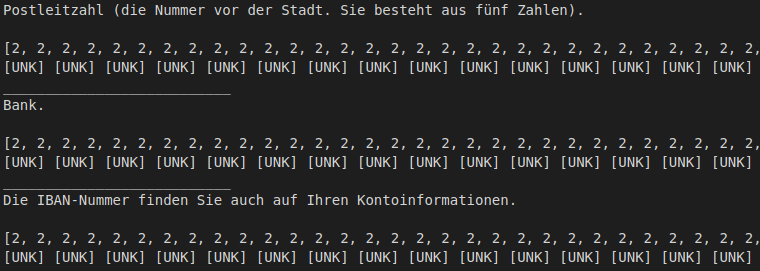
\includegraphics[scale=0.7]{images/NMT_lr1e-4_Ausgabe.png}
	\caption{NMT-Model Ausgabe bei einer LR von 1e-4}
	\label{fig:NMT_Ausgabe}
\end{figure}

In der \cref{fig:NMT_Ausgabe} sind 6 Beispiele ersichtlich, die aus dem Testkorpus ausgewählt wurden. Die Gruppierung erfolgt in zwei Paaren. Die Listen in \cref{fig:NMT_Ausgabe} repräsentieren die Prognose des Modells und die Sätze unterhalb der Zahlenlisten sind Target-Sätze. Die Prognose besteht aus der wiederholten Token-Id 2. Die Id repräsentiert den Token \textit{[UNK]}, welcher dafür verwendet wird, unbekannte Wörter, bzw. solche die nicht in der Look-up-Tabelle vorkommen, zu ersetzen. 


Im zweiten Test konnte das gleiche Ergebnis wie bei der \cref{fig:NMT_Ausgabe} festgestellt werden. Die Prognosen unterscheiden sich nicht von dem Modell, das mit der Lernrate von 1e-4 gelehrt wurde. In \cref{fig:NMT_Ausgabe1e-3} können die Prognosen eingesehen werden.

%TODO: NEW
\begin{figure}
	\centering
	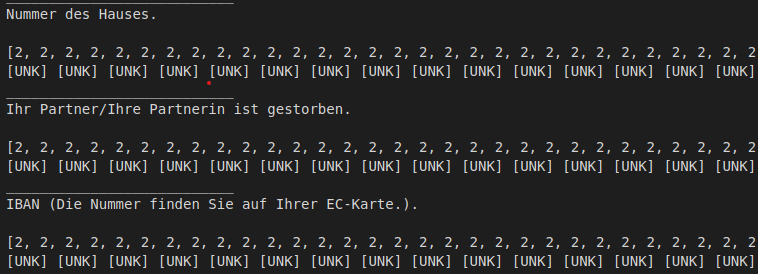
\includegraphics[scale=0.7]{images/NMT_lr1e-3_Ausgabe.png}
	\caption{NMT-Model Ausgabe bei einer LR von 1e-3}
	\label{fig:NMT_Ausgabe1e-3}
\end{figure}

Die Prognose des Modells besteht ausschließlich aus den Token \text{\quotedblbase [UNK]\quotedblbase}.

Anhand dieser Betrachtungen kann entschlossen werden, dass das Modell fehlerhaft konvergiert.


\subsection{Schlussfolgerung}
Der Grund für die Divergenz konnte nicht festgestellt werden. Die Eingaben wurden überprüft und zeigten keine Mängel.

Aus den Testergebnissen und der Eingabeuntersuchung kann hergeleitet werden, dass das Modell mit der vorliegenden Struktur ungeeignet für die anzustrebende Aufgabe ist. Im folgenden Kapitel wird ein gelungeneres Modell vorgestellt (besser im Sinne von Prognosequote und Konvergenz).

\section{Seq2Seq Model}

Das nächste Modell, das untersucht wurde, ist ein Sequenz-to-Sequenz-Model (seq2seq Model). Wie der Name andeutet, liefert das Modell eine entsprechende Antwortsequenz für jede beliebige Sequenz. Solche Modelle werden für Textgeneratoren verwendet, sind aber auch für Übersetzungsaufgaben geeignet. Die Idee ist, das Modell für die Aufgabe \text{\quotedblbase Übersetzung in einfache Sprache\quotedblbase} anzupassen. Wie genau das erfolgt, wird in den nächsten Kapiteln vorgestellt.

\subsection{Struktur}
Laut \cite{NMT&ATT:22} ist das Modell ein Neural Machine-Translation-Model und bezeichnet ein System, das die Wahrscheinlichkeit $p(y|x)$ für eine beliebige Sequenz $x_1$, \dots, $x_n$ berechnet, zu einer anderen $y_1$, \dots, $y_m$ zugeordnet zu werden. Das Modell besteht aus einem Encoder und einem Decoder. Der Encoder berechnet die Vektor-Repräsentation für jede Sequenz \textit{s} und der Decoder erzeugt die Wörter schrittweise. Die Funktion, die vom Decoder berechnet wird, ist die bedingte Wahrscheinlichkeit:

\begin{equation}
	logp(x|y) = \sum_{j=1}^m logp(y_j|y_{<j}, s) \cite{NMT:2017}
\end{equation}

Eine solche Zerlegung kann im Decoder mit Hilfe von Recurrent-Neural-Networks (RNN) modeliert werden. In der Literatur verwendet man unterschiedliche RNNs, was wiederum zu unterschiedlichen Ergebnissen führt. In diesem Kapitel wird das übliche Modell mit jeweils einem RNN für den Encoder und Decoder thematisiert. Ein zweites Modell wird gebaut, damit ein vortrainiertes BERT-Modell für den Encoder verwendet werden kann. So ein Prinzip nennt sich Transfered Learning \cite{transfered_learning:22}. Transfered Learning beschreibt den Prozess, in wessen Rahmen die erworbene Information aus unbeschrifteten Daten verwendet wird, um beschrifteten kleineren Datensatz zu bearbeiten. Das soll die Inferenz aus dem kleinen Datensatz verbessern, sodass der Lernprozess zu besseren Ergebnissen führt. 

Die Struktur des Modells wird in der \cref{fig:NMT_Model} ersichtlich:

\begin{figure}[H]
	\centering
	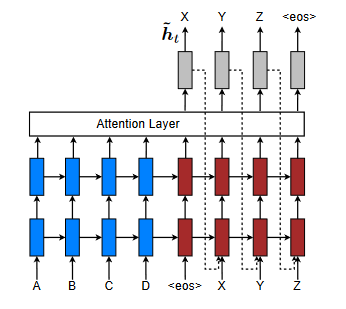
\includegraphics[scale=0.85]{images/NMT-Model.png}
	\caption{NMT-Model Struktur \cite{NMT:2017}}
	\label{fig:NMT_Model}
\end{figure}

Die blauen Rechtecke repräsentieren den Encoder und die Roten dementsprechend den Decoder. Der übliche Encoder bearbeitet die Wörter aus der Sequenz schrittweise, jedoch ergibt sich in unserem Fall, bedingt durch die verwendete Quelle \cite{NMT&ATT:22}, dass die Sequenz komplett betrachtet wird, woraus der Encodervektor entsteht.

Der Encoder für dieses Modell ist der BERT-base-german-cased-Model, der auf Huggingface \cite{bert_based:19} zu finden ist. Das nächste Unterkapitel setzt sich mit dem Decoder auseinander.

\subsection{Decoder}
Das Hauptziel des Decoders ist, die Prognose für den nächsten Token zu bestimmen. Die Operationen im Decoder können in 5 Schritte aufgeteilt werden \cite{NMT&ATT:22}:
\begin{enumerate}\label{steps_BNMT}
	\item es wird der Targetvektor geliefert
	\item ein RNN markiert die aktuell erzeugten Tokens
	\item die Ausgabe vom RNN ist die Eingabe in der Attention-Schicht und es wird der Kontextvektor geliefert
	\item der Attentionsvektor wird generiert
	\item die neuen Prognosen für den Token werden dem Attentionvektor entnommen.
\end{enumerate}

Der Decoder bringt Attention ein und beachtet somit besondere Abschnitte aus der Eingabesequenz. In der Attention-Schicht fließt eine Sequenz aus Vektoren und für jeden Sequenzvektor wird ein Attentionsvektor geliefert. Anschließend wird der Attentionsvektor in den Kontextvektor umgewandelt. Schließlich wird der Kontextvektor transformiert, sodass ein Logits-Vektor erhalten wird, dessen Größe gleich die Anzahl der Wörter im Corpus ist.

Der Attentionvektor wird mittels der folgenden Formel berechnet:

\begin{equation}
	a_{t}(s) = \frac{\exp(score(h_t, \overline{h}_s))}{\sum^{S}_{s'=1} \exp(score(h_t, \overline{h}_{s'})) } \cite{NMT:2017}
\end{equation}

Die Formel ist wie folgt zu lesen: \textit{t} steht für den Decoder- und \textit{s} für den Encoderindex. Die Variable $a_{ts}$ ist die Attentionweights. $h_t$ bezeichnet den Decoderzustand und $h_s$ den aktuelle Zustand vom Encoder. Weiterhin ist die \textit{score}-Funktion gegeben \cite{NMT:2017}:

\begin{equation} \label{score_func}
	score(h_t, \overline{h}_s) = 
	\begin{cases}
		h_t^\top \overline{h}_s & \textit{dot} \\
		h_t^\top W_a \overline{h}_s & \textit{general} \\
		v_a^\top \tanh(W_a[h_t^\top;\overline{h}_s]) & \textit{concat}
	\end{cases}
\end{equation}
Hier sind $W_a$ und $v_a$ Variablen, die gelernt werden müssen. Die zweite und die dritte Varianten (\textit{general} und \textit{concat}) wurden zum Gegenstand der praktisch-experimentellen Testphase für die Berechnung des Kontextvektors. Im Kontextvektor befindet sich die Information über die Wichtigkeit der einzelnen Ausgangswörter für das Targetwort. Anhand des Kontextvektors wird die Prognose geliefert.

Als nächstes wird im \cref{BSLM_imp} die Implementierung für das Modell erläutert.

\subsection{Implementierung} \label{BSLM_imp}
Das Modell besteht aus zwei Bestandteilen, der Encoder und der Decoder. Für die Analyse wird mit drei unterschiedlichen Modellen gearbeitet. Zwei davon setzen ein vortrainiertes BERT-Modell als Encoder ein. Das dritte Modell besteht aus einer RNN-Schicht, ähnlich wie im Decoder.

\subsection{Implementierung vom Encoder im NMT-Model ohne BERT}
Der Encoder im NMT besteht aus zwei Schichten. Die Implementierung ist gegeben:
\begin{lstlisting}
	self.embedding = Embedding(self.vocab_size, enc_units)
	
	self.gru = GRU(self.enc_units, return_sequences=True, return_state=True, recurrent_initializer='glorot_uniform')
\end{lstlisting}

Der Encoder hier besitzt keine positionelle Einbettung im Vergleich zum Encoder des Transformers (s. \cref{Transformer_Enc_class}) oder BERT (s. \ref{bert_class}). Dieser Unterschied kann im Gegensatz zum Modell, das BERT für den Encoder einsetzt, in der Testphase eine Rolle spielen.


\subsubsection{Implementierung vom Decoder}
Der Decoder wird nach den 5 Schritten aus \ref{steps_BNMT} implementiert und folgender Programmabschnitt stellt diese dar:
\begin{lstlisting}[language=Python, caption={NMT-Decoder}, label={BNMT_Decoder}]
	# For Step 1. The embedding layer converts token IDs to vectors
	self.embedding = Embedding(self.vocab_size, d_model)
	
	# For Step 2. The RNN keeps track of what's been generated so far.
	self.gru = GRU(d_model, return_state=True, return_sequences=True, recurrent_initializer='glorot_uniform')
	
	# For Step 3. The RNN output will be the query for the attention layer
	self.attention = BahdanauAttention(self.d_model)
	# oder 
	# self. attention = LuongAttention(self.d_model)
	
	# For Step 4. converting `ct` to `at`
	self.Wc = Dense(self.d_model, activation=tf.math.tanh, use_bias=False)
	
	# For Step 5. This fully connected layer produces the logits for each output token
	self.fc = Dense(self.vocab_size)
\end{lstlisting}

Für den zweiten Schritt können auch andere RNNs benutzt werden, unter Anderem auch eine \textbf{LSTM}-Schicht (\textbf{L}ong \textbf{S}hort \textbf{T}erm \textbf{M}emory). Im Schritt drei wird in diesem Fall die Bahdanau-Attention verwendet, die zweite Option wäre die Luong's Multiplikative Attention, der Unterschied in der Funktionen ist in der \cref{score_func} zu sehen.

\section{Erkenntnisse} \label{BSLM_analysis}

In diesem Kapitel werden drei Modelle getestet - zwei BERT-basierte NMT-Modelle mit unterschiedlichen Score-Funktionen und ein NMT-Modell (Transformer-ähnliches Modell) ohne die Verwendung von BERT (mit der Bahndanau's additive Attention). Die Modelle werden für 100 Iterationen trainiert und es werden vier unterschiedliche Lernraten geprüft - 0.001, 0.0001, 0.00002, 0.00001. Der verwendete Optimizer ist Adam (Adaptive Moment Estimation).

Für Trainingsdaten wird dasselbe Corpus (s. \cref{corpus_def}) genommen.

Ziel der Tests ist es das beste Modell zu bestimmen. Der Test hilft beim Erkunden der besten Lernrate und Bestimmung des Modells, das die Aufgabe \text{\quotedblbase Übersetzung in einfache Sprache\quotedblbase} am besten löst. Als Kriterium dafür werden das BLEU-Score und ausgewählte Ein- und Ausgabe der Modelle angewendet.

Die drei Modelle besitzen auch unterschiedliche Anzahl an Variablen:
\begin{itemize}
	\item Das Simple Language Model besitzt 78 598 704 Variablen
	\item Das BERT Simple Language Model mit Bahdanaus Attention besitzt 161 096 496
	\item Das BERT Simple Language Model mit Luongs Attention besitzt 159 914 544.
\end{itemize}

Die zwei BERT-Modelle sind doppelt so komplex wie das Simple-Language-Modell. Ob das ein Vorteil, oder Nachteil ist, zeigt sich in den Tests.

\subsection{Training auf einem High Performance Computer}

Die Experimente werden auf einem Hochleistungsrechner in Kaiserslautern durchgeführt. Die Modelle trainieren auf dem 'Elweritsch'-Cluster (\cite{AHRP:2022}) im TU Kaiserslautern. Die Untersuchungen werden mit den Lernraten (0.001, 0.0001, 0.00002, 0.00001) durchgeführt. Für die letzte Lernrate werden nur Tests für die BERT-Modelle ausgeführt. Zum Trainieren wird das in \cref{corpus_def} eingeführte Corpus verwendet. Für die Evaluierung wurden sowohl das Trainingscorpus als auch ein zusätzliches Corpus, das aus 10 Evaluierungspaaren besteht, benutzt. Alle Lernprozesse haben 100 Iterationen durchlaufen, außer den Tests mit der Lernrate 0.00001, die für 3 Phasen von jeweils 50 Iterationen durchlaufen haben.

Die Abbildungen, die als Nächstes dargestellt werden, zeigen in ihrer X-Achse die Anzahl der Iterationen, und in der Y-Achse werden die Werte für die Fehlerrate angegeben. Der Batch hat für alle Tests den Wert von 1. Das bedeutet, dass pro Iteration jeweils ein Trainingspaar bearbeitet wird.

\subsubsection{Testen mit Lernrate 0.001}
Als erstes wird die Lernrate von \textbf{0.001} angewendet. Die \cref{NMT_lr1e-3,BNMT_Bahdanau_lr1e-3,BNMT_Luong_lr1e-3} zeigen den Lernprozess. Aus den Abbildungen kann ein besseres Verständnis dafür verschafft werden, wie geeignet eine niedrigere Fehlerrate für die gegebenen Größen der Modelle ist.


\begin{figure}[p]
	\centering
	\begin{subfigure}[H]{\textwidth}
		\centering
		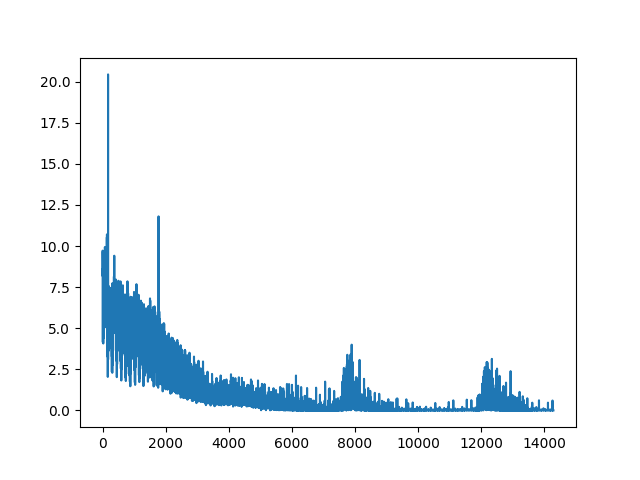
\includegraphics[scale=0.55]{images/slm_1e-3_100EP_v5.png}
		\caption{SLM-Model mit Lernrate 0.001}
		\label{NMT_lr1e-3}
	\end{subfigure}
	\begin{subfigure}[H]{\textwidth}
		\centering
		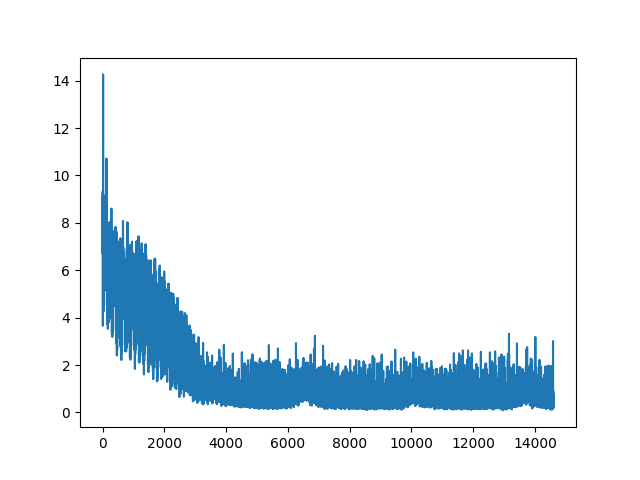
\includegraphics[scale=0.55]{images/bslm_bahdanau_1e_3_100EP.png}
		\caption{BSLM-Model(Bahndanau)}
		\label{BNMT_Bahdanau_lr1e-3}
	\end{subfigure}
	\begin{subfigure}[H]{\textwidth}
		\centering
		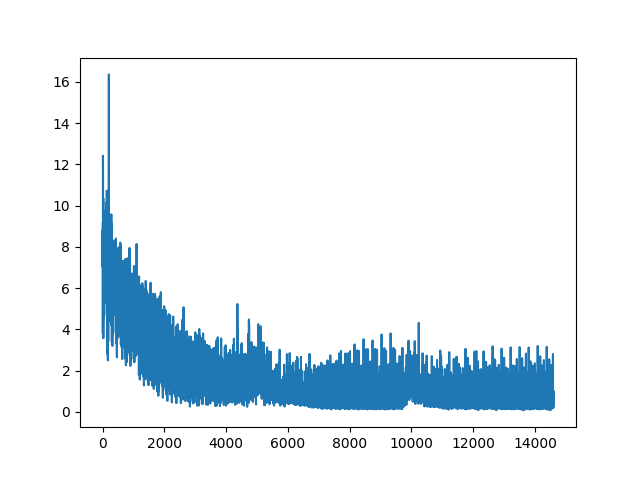
\includegraphics[scale=0.55]{images/bslm_luong_100EP_1e-3.png}
		\caption{BSLM-Model (Luong)}
		\label{BNMT_Luong_lr1e-3}
	\end{subfigure}
	
	\caption{Fehlerwerte bei den Tests mit der Lernrate 0.001}
	\label{fig:three graphs}

\end{figure}
Laut \cref{NMT_lr1e-3} wird den Optimalzustand der Variablen schon bei dem Iterationsschritt 10000 erreicht. Innerhalb der ersten 3000 Iteraionen erfolgen die größten Verbesserungen des Modells und schätzungsweise ab dem Schnittpunkt von 10 000 können nur minimale Verbesserungen festgestellt werden. Danach steigen die Fehlerwerte der Modelle für einige Schritte sogar, aber in den letzen Epochen verbessert sich der Durchschnitt und es wird eine Fehlerquote von nahezu 0 erreicht. 

Die letzten \cref{BNMT_Luong_lr1e-3,BNMT_Bahdanau_lr1e-3} zeigen deutlich höhere Fehlerwerte als in der \cref{NMT_lr1e-3}. In Bezug auf die Fehlerwerte weist das Simple-Language-Modell die größte Verbesserung. Ob niedrige Fehlerwerte gleichbedeutend mit einem guten Modell sind, zeigt sich später bei der Untersuchung mit unbekannten Corpussätzen.

\subsubsection{Testen mit Lernrate 0.0001}

Die \cref{NMT_lr1e-4,BNMT_Bahdanau_lr1e-4,BNMT_Luong_lr1e-4} zeigen eine stetige Verbesserung. Wenn die Fehlerwerte als Kriterium verwendet werden, könnte man sagen, dass das beste Modell wieder das SLM-Modell sei:
\begin{figure}[H]
	\centering
	\begin{subfigure}[b]{\textwidth}
		\centering
		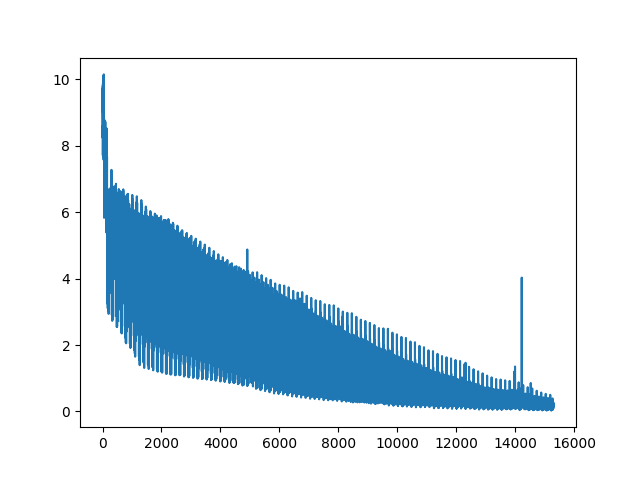
\includegraphics[scale=0.55]{images/slm_1e-4_101EP.png}
		\caption{SLM-Model}
		\label{NMT_lr1e-4}
	\end{subfigure}
	\begin{subfigure}[b]{\textwidth}
		\centering
		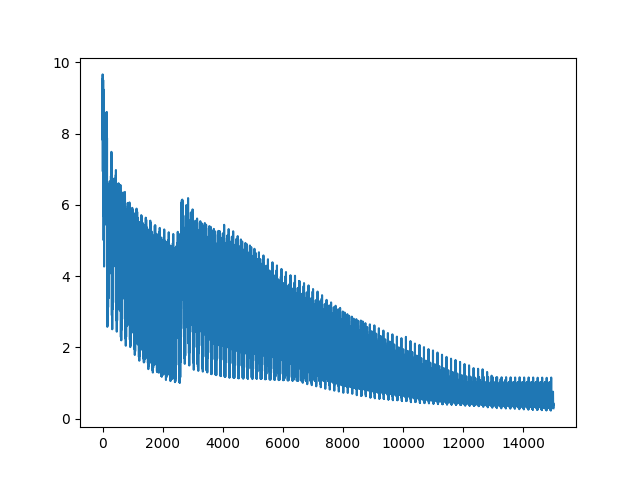
\includegraphics[scale=0.55]{images/bslm_bahdanau_1e_4_100EP.png}
		\caption{BSLM (Bahdanau)}
		\label{BNMT_Bahdanau_lr1e-4}
	\end{subfigure}
	\caption{Fehlerwerte bei den Tests mit der Lernrate 0.0001}
	\label{fig:lr_0001}
\end{figure}
\begin{figure}
	\centering
		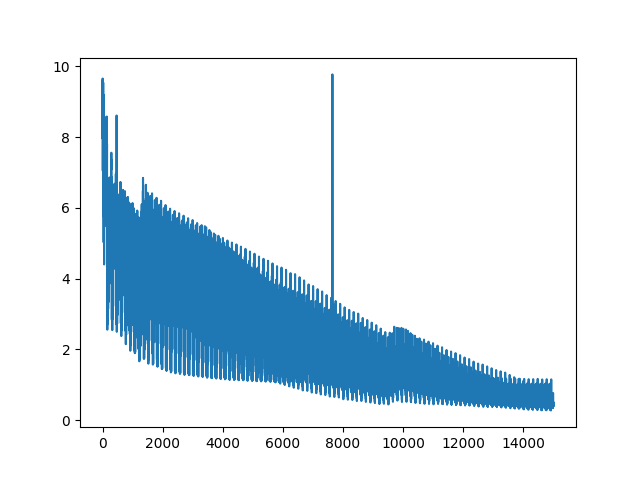
\includegraphics[scale=0.55]{images/bslm_luong_100EP_1e-4.png}
		\caption{ Fehlerwerte bei den Tests mit der Lernrate 0.0001 (Fortsetzung - BSLM (Luong))}
		\label{BNMT_Luong_lr1e-4}

\end{figure}


Die Kurve der Fehlerfunktion für die Modelle BSLM (Bahdanau und Luong) sieht sehr ähnlich aus, jedoch könnte keinem der Modelle ein Vorteil zuerkannt werden. Ab dem 13 000. Schritt ist ein Minimum erreicht, das durch die restlichen Iterationen kaum verbessert wird. Aus den Ausgaben der Tests wird jedoch in den späteren Iterationen trotzdem eine Verbesserung erzielt.
 

\subsubsection{Testen mit 0.00002}
Der letzte Test wird mit der Lernrate von \textbf{0.00002} durchgeführt. In den 
\cref{NMT_lr2e-5,BNMT_Bahdanau_lr2e-5,BNMT_Luong_lr2e-5} kann der Verlauf des Trainingsprozesses verfolgt werden. 

%TODO: Die Figuren noch anpassen

	
	\begin{figure}[H]{\textwidth}
		\centering
		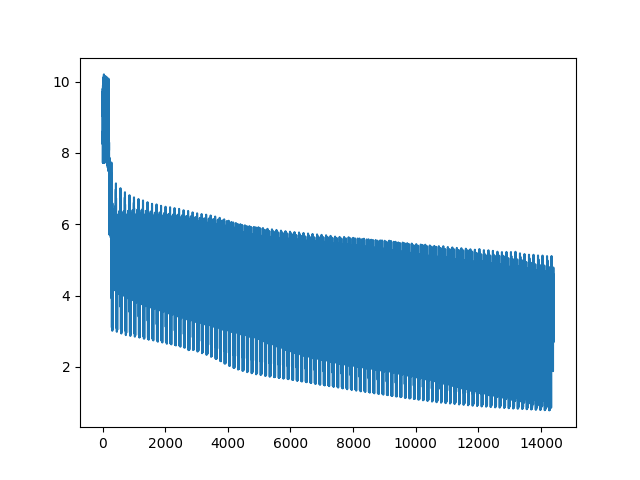
\includegraphics[scale=0.55]{images/slm_101EP.png}
		\caption{Fehlerwerte bei den Tests mit der Lernrate 0.00002 (SLM-Model)}
		\label{NMT_lr2e-5}
	\end{figure}
\begin{figure}[H]
	\centering
	\begin{subfigure}[b]{\textwidth}
		\centering
		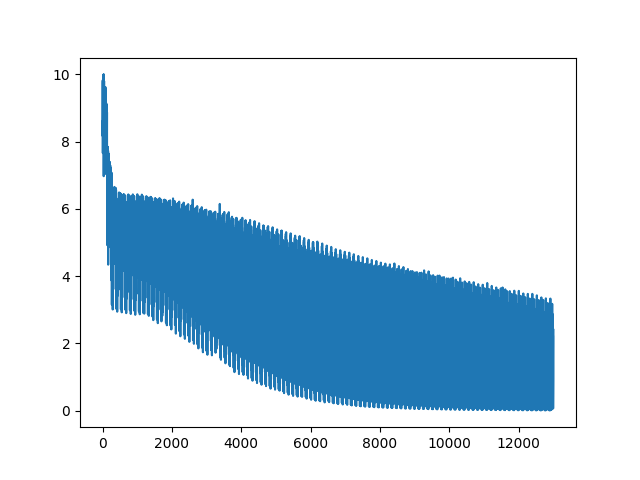
\includegraphics[scale=0.55]{images/bslm_bahdanau_2e_5_100EP_v4.png}
		\caption{BSLM (Bahdanau)}
		\label{BNMT_Bahdanau_lr2e-5}
	\end{subfigure}
	\begin{subfigure}[b]{\textwidth}
		\centering
		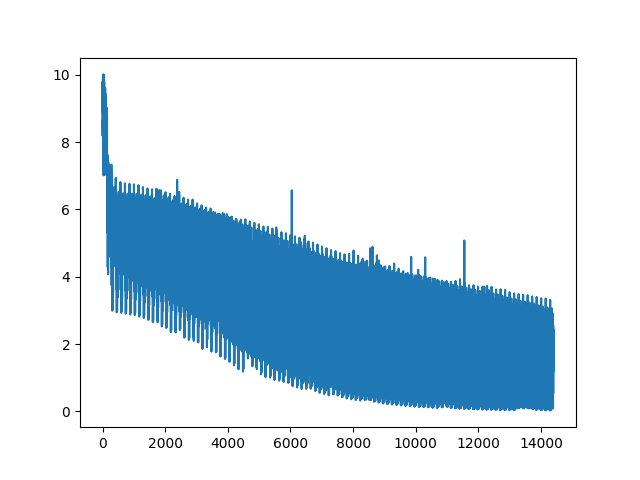
\includegraphics[scale=0.55]{images/bslm_luong_100EP_2e-5_V4.png}
		\caption{BSLM (Luong)}
		\label{BNMT_Luong_lr2e-5}
	\end{subfigure}
	
	\caption{Fehlerwerte bei den Tests mit der Lernrate 0.00002 (Fortsetzung)}
	\label{fig:lr_00002}
\end{figure}


Die ersten Hundert Iterationen weisen die größte Optimierung der Fehlerfunktion auf. Außerdem kann ein klarer Vorteil der BERT-Modelle erkannt werden. Mit der Senkung der Lernrate steigen die Fehlerwerte, aber die BERT-Modele stellen ihre Fähigkeiten unter Beweis, trotz der größeren Anzahl an Variablen.

\subsubsection{Testen mit 0.00001}

Im Laufe der Untersuchung konnte aus den Ausgaben der BERT-Modelle festgestellt werden, dass die Senkung der Lernraten bei den dargestellten BERT-Modellen bessere Ergebnisse zu Folge hatte. Die ausgewählten Beispiele aus dem \cref{bert_guesses} bestätigen diese Behauptung. Der Kandidat \text{\quotedblbase Anrede\quotedblbase} wurde als Beispiel genommen, da er in allen Testdurchläufen eingebracht wurde.
%TODO: Das Hier ist neu und Umlaute aus dem Listings werden nicht angezeigt im PDF
\begin{lstlisting}[label=bert_guesses,caption={Prognose für ausgewählte Eingaben der BERT-Modelle}]
	Candidate: Anrede
	Target: Herr oder Frau.
	# BSLM_HPC_General_lr1e-3
	Prediction: ['Ich', 'mache', 'mir', 'einen', 'Kaffee']
	
	# BSLM_HPC_General_lr1e-4
	Prediction: ['Sie', 'sind', 'schwanger', '.']
	
	# BSLM_HPC_General_lr2e-5
	Prediction: ['Herr', 'oder', 'Frau', '.']
	
	# BSLM_HPC_Bahdanau_lr1e-3
	Prediction: ['Ich', 'mag', 'hier', 'zu', 'sein', '.', 'Die', 'Natur', 'ist', 'sehr', 'schön', 'und', 'die', 'Luft', 'ist', 'sehr', 'frisch', '.', 'Ich', 'fühle', 'keine', 'Probleme', 'hier', '.', 'Ich', 'fühle', 'mich', 'auch', 'frei', '.']
	
	# BSLM_HPC_Bahdanau_lr1e-4
	Prediction: ['Wir', 'wollen', 'morgen', 'in', 'die', 'Stadt', 'gehen', '.']
	
	#BSLM_HPC_Bahdanau_lr2e-5
	Prediction: ['Herr', 'oder', 'Frau', '.']
\end{lstlisting}

Als weitere Beobachtung konnte aus manchen Ausgaben Overfitting (s. \cref{overfitting}) nachgewiesen werden. Dies hatte zu Folge, dass zwei weitere Tests bestehend aus 3 Phasen als notwendig erachtet wurden. Die Entscheidung, das Lernen in drei Phasen aufzuteilen, kam nach der Evaluierung der anderen Lernraten. Die Modelle wiesen zwar ein gutes Minimum der Fehlerfunktion (s. \cref{NMT_lr1e-3,BNMT_Bahdanau_lr1e-3,BNMT_Luong_lr1e-3}) auf, jedoch zeigten sie bei unbekannten Sätzen sinnfreie Übersetzungen. Durch die Phasentrennung wird die Lösung dieses Problems angestrebt.

\begin{lstlisting}[label=overfitting,caption={Beispiele für Overfitting}]
	Candidate: Antragstellende Person
	Target: Wer stellt den Antrag?
	
	# SLM_HPC_v1_without_BERT_lr1e-3
	Prediction: ['Nummer', 'von', 'der', 'Renten', '##versicherung', '.']
	
	# SLM_HPC_v1_without_BERT_lr1e-4
	Prediction: ['Sie', 'haben', 'eine', 'Frau', 'geheiratet', '.']
	
	# BLM_HPC_v1_lr1e-3_Bahdanau_100EP
	Prediction: ['Ich', 'mag', 'hier', 'zu', 'sein', '.', 'Die', 'Natur', 'ist', 'sehr', 'schön', 'und', 'die', 'Luft', 'ist', 'sehr', 'frisch', '.', 'Ich', 'fühle', 'keine', 'Probleme', 'hier', '.', 'Ich', 'fühle', 'mich', 'auch', 'frei', '.']
	
	Candidate: Stellung in Beruf?
	Target: Was machen Sie?
	# SLM_HPC_v1_without_BERT_lr1e-4
	Prediction: ['Sie', 'haben', 'eine', 'Frau', 'geheiratet', '.']
	
	# BLM_HPC_v1_lr1e-3_Bahdanau_100EP
	Prediction: ['Ich', 'mag', 'hier', 'zu', 'sein', '.', 'Die', 'Natur', 'ist', 'sehr', 'schön', 'und', 'die', 'Luft', 'ist', 'sehr', 'frisch', '.', 'Ich', 'fühle', 'keine', 'Probleme', 'hier', '.', 'Ich', 'fühle', 'mich', 'auch', 'frei', '.']
\end{lstlisting}

In den beiden Tests laufen die Bahdanau- und Luong-Modele für 3 Phasen á 50 Iterationen und in \cref{BSLM_Bahdanau_lr1e-5_50EP,BSLM_Luong_lr2e-5_50EP} ist die Fehlerfunktion für die letzten 50 Iterationen aufgezeichnet.

%TODO: New

	\begin{figure}[H]
		\centering
		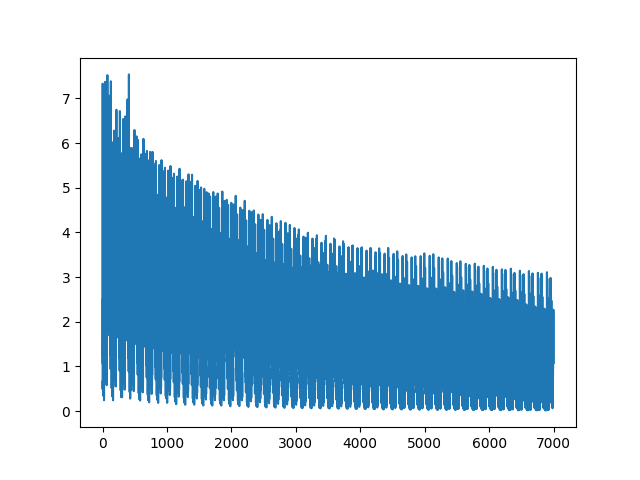
\includegraphics[scale=0.55]{images/bslm_bahdanau_2e_5_50EP_P3.png}
		\caption{Fehlerwerte bei den Tests mit der Lernrate 0.00001 (Bahdanau-Model)}
		\label{BSLM_Bahdanau_lr1e-5_50EP}
	\end{figure}
	\begin{figure}[H]
		\centering
		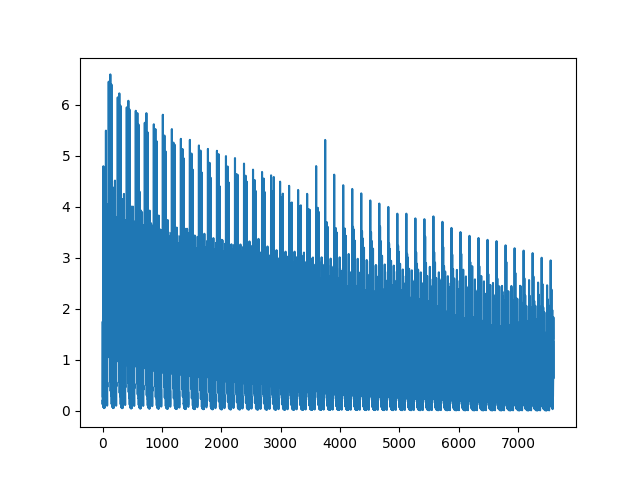
\includegraphics[scale=0.55]{images/bslm_luong_50PT3_2e-5.png}
		\caption{Fehlerwerte bei den Tests mit der Lernrate 0.00001 (Luong-Model)}
		\label{BSLM_Luong_lr2e-5_50EP}
	\end{figure}
	
	\caption{Fehlerwerte bei den Tests mit der Lernrate 0.00001}
	\label{fig:lr_00001}


Aus der \cref{BSLM_Bahdanau_lr1e-5_50EP,BSLM_Luong_lr2e-5_50EP} geht hervor, dass das Bahdanau-Model kleinere Fehlerwerte und geringere Schwankung zeigt. Die Lernkurven sprechen für die Lernfähigkeit des Bahdanau-Modells. Die Schwankung der Kurve erklärt sich durch die Zufälligkeit bei der Auswahl der Trainingspaare. Das hat sich als eine gute Strategie erwiesen, was entsprechende Ergebnisse bei der Untersuchung mit BLEU erbracht hat.

\subsection{BLEU-Score}

BLEU ist kurz für \textbf{B}i-\textbf{L}ingual \textbf{E}valuation \textbf{U}nderstudy und ist ein Berechnungsmodell zur schnellen und automatischen Evaluierung der Übersetzungen eines Modells. Für diesen Zweck werden Methoden aus der Bibliothek \textit{nltk.translate} angewendet. 

Die Berechnung des BLEU-Score erfolgt, indem der gewichtete geometrische Durchschnitt (\cref{geometric_mean}) aus den N-Gramm-Werten in allen Rangordnungen von 1 bis n errechnet wird \cite{BLEU:17}.

\begin{equation}\label{geometric_mean}
	\left(\prod_{i=1}^{n} x_i^{w_i}\right)^{\frac{1}{\sum_{i=1}^{n} w_i}} \cite{weighted_geometric_mean:22}
\end{equation} 

%TODO:NEW
In der \cref{geometric_mean} bezeichnet $x_i \in \mathbb{R}$ ein N-Gramm-Wert der Rangordnung $i$. Der N-Gramm $x_i$ ergibt sich aus der Abdeckung von einer fragmentierten Target-Einheit und einem fragmentierten Kandidaten. Die Zahl n stellt die Anzahl der betrachteten Fragmente dar. Üblicherweise wird für n der Wert 4 eingesetzt. Der Wertebereich von $x_i$ liegt zwischen 0 und 1, sodass $x_i$ bei voller Übereinstimmung den Wert 1 und bei fehlender den Wert 0 erhält. Die Kandidaten dürfen auch partiell die Target-Einheit abdecken. In diesem Fall erhält $x_i$ einen rationalen Wert. Die Variable $w_i$ repräsentiert das Gewicht der Ordnung $i$. Üblicherweise wird der Wert $w$ gleich $\frac{1}{n}$ in allen Rangordnungen ausgewählt, um sicherzustellen, dass alle n-Gram-Werte gleichermaßen zum gesamt Score beitragen.

Als nächstes wird der BLEU-Score der Modelle untersucht. In der \cref{bleu_score} sind die BLEU-Werte in absteigender Reihe gegeben:

%TODO: Update this graphic
\begin{figure}[H]
	\centering
	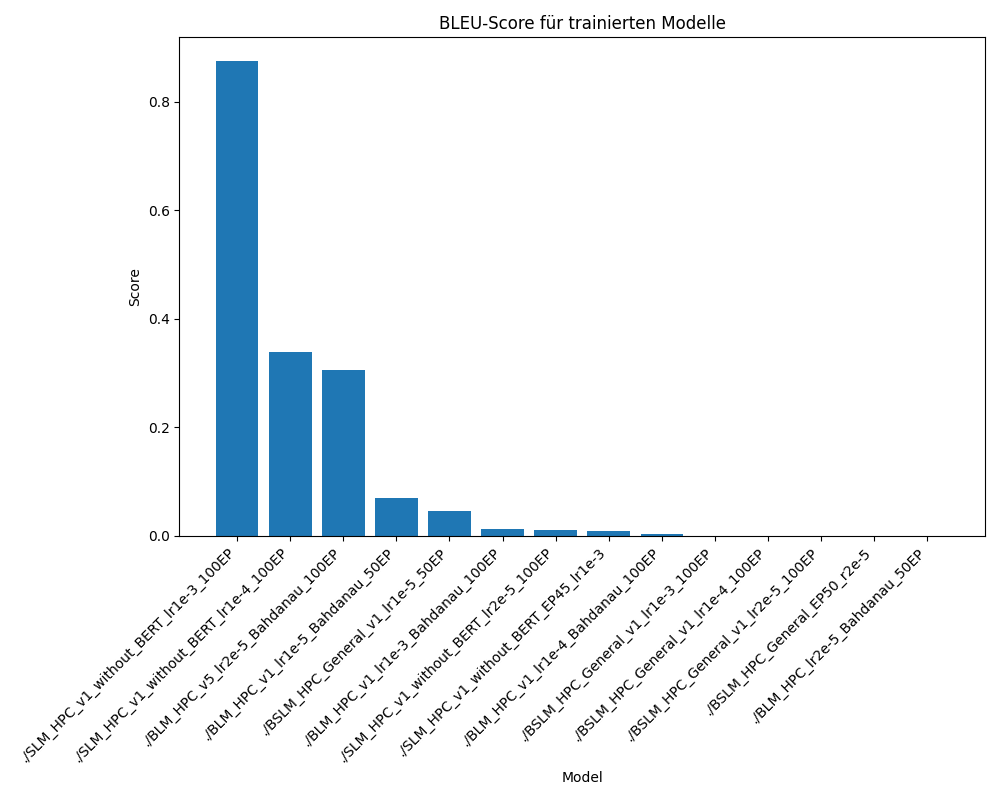
\includegraphics[scale=0.55]{images/bleu_scores_4.png}
	\caption{BLEU-Scores}
	\label{bleu_score}
\end{figure}

Interessanterweise weisen die SLM-Modele ohne BERT den besten Wert auf. Die am wenigsten zufriedenstellend bei der Übersetzung sind die BSLM-Modelle, bei welchen die \textit{general}-Funktion (siehe \cref{score_func}) verwendet wird. Hierzu muss man anmerken, dass der BLEU-Score auf den ganzen Traningsdaten basiert.

Eine weitere Erkenntnis aus den Lernprozessen und \cref{bleu_score} ist, dass die BERT-Modelle sich besser mit kleineren Lernraten entwickeln, während das simple Modell besser auf die höheren Lernraten reagiert. Die Beispiele im \cref{bert_guesses,nmt_guesses} bestätigen diese These. Die Prognosen werden aus dem BLEU-Test mit dem Trainingssatzes ausgeschrieben. Die Ausgabe werden für die Eingabe \text{\quotedblbase Anrede\quotedblbase} ausgesucht.

\begin{lstlisting}[label=nmt_guesses, caption={Prognosen von Simple-Language-Model}]
	Candidate: Anrede
	Target: Herr oder Frau?
	# SLM_HPC_ohne_BERT_lr2e-5
	Prediction: ['In', '##name', '.']
	
	# SLM_HPC_ohne_BERT_lr1e-4
	Prediction: ['Herr', 'oder', 'Frau', '.']
	
	# SLM_HPC_ohne_BERT_lr1e-3
	Prediction: ['Herr', 'oder', 'Frau', '.']
\end{lstlisting}

Zur Bestimmung der eigentlichen Anwendbarkeit der Modelle wird ein unbekannter Datensatz erstellt und in einem weiteren BLEU-Test verwendet. Im nächsten Kapitel wird ein Graph mit den Ergebnissen aufgeführt.

\subsubsection{Untersuchung mit Evaluierungsdaten}

Zu Bekräftigung der gewonnenen Erkenntnisse wird eine zusätzliche Untersuchung mit Sätzen, die nicht in dem Trainingscorpus vorkommen, durchgeführt. Das Ziel ist es, die Anwendbarkeit der Modelle zu prüfen und festzustellen, ob sie mit einem kleinen Corpus (\cref{corpus_def}) gelehrt werden können, sowie ob sie schlussendlich für einen Produktionseinsatz geeignet sind. Die \cref{bleu_score_unseen} zeigt die Scores der Modelle:

%TODO:Aktualisiere die Abbildung mit den Modellen 2e-5 50EP
\begin{figure}[H]
	\centering
	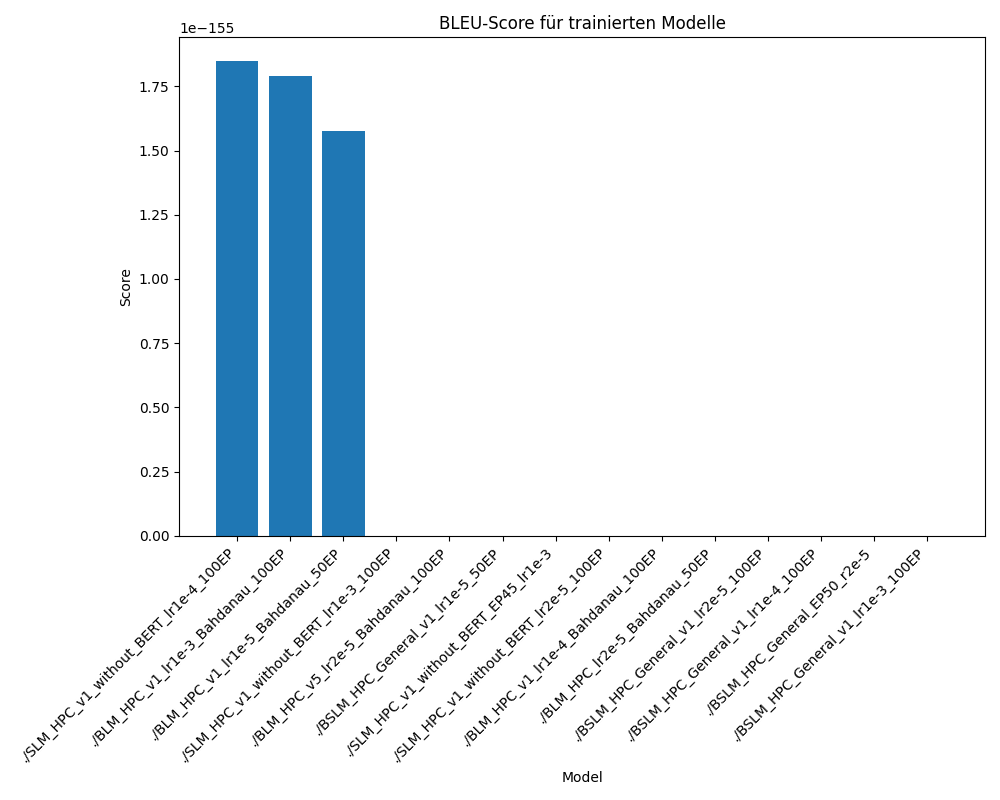
\includegraphics[scale=0.55]{images/bleu_scores_unseen_4.png}
	\caption{BLEU-Scores für unbekannte Sätze}
	\label{bleu_score_unseen}
\end{figure}

Bei diesem Test enttäuschen alle Modelle. Bemerkenswert ist, dass die besten Modelle laut \cref{bleu_score_unseen} das SLM mit Lernrate 0.0001 und zwei BERT-Modelle mit Bahdanau Attention mit Lernrate 0.001 und 0.00001. Auffallend ist, dass sich in den unterschiedlichen Testläufen jeweils andere Modelle als die Besten erwiesen haben.


\subsection{Schlussfolgerung}
Aus den \cref{bleu_score,bleu_score_unseen} zeigte sich, dass sich das Simple-Language-Model zwar als bestes Modell qualifizieren konnte, aber es scheiterte bei dem unbekannten Corpus, gleichermaßen wie alle anderen Modelle. Somit konnte keins der Modelle den Test mit dem unbekannten Corpus bestehen. Die BLEU-Tests rechtfertigten die niedrigen Erwartungen, weil die Lernprozesse zeigten, dass die Modelle bei dem Evaluierungsabschnitt fehlerhafte Prognosen geliefert haben. Angesichts des verwendeten kleinen Corpus ist es nicht möglich, ein funktionstüchtiges Modell zu trainieren. Die Hypothese war, dass der BERT-Encoder die kleine Größe des Corpus kompensieren würde, leider geht aus den Tests das Gegenteil hervor. 

Ein größeres Corpus sollte für die vorliegende Aufgabe (Übersetzung in einfache Sprache) verwendet werden, um die Ergebnisse zu verbessern, oder idealerweise zum Erfolg zu führen. Es ist nicht möglich ein Modell zum Zweck der Übersetzung in einfache Sprache mit einem nicht ausreichenden, lediglich aus 168 Datensätzen bestehenden Corpus zu trainieren.

%\subsubsection{Die besten Modele}
%Als nächstes werden die Lernkurven in \cref{SLM_lr1e-3,BSLM_Bahdanau_lr2e-5,BSLM_Luong_lr2e-5} für die besten Modele jeder Art dargestellt nach dem BLEU-Score aufgestellt. 
%
%\begin{figure}
%	\centering
%	\begin{subfigure}[b]{0.3\textwidth}
%		\centering
%		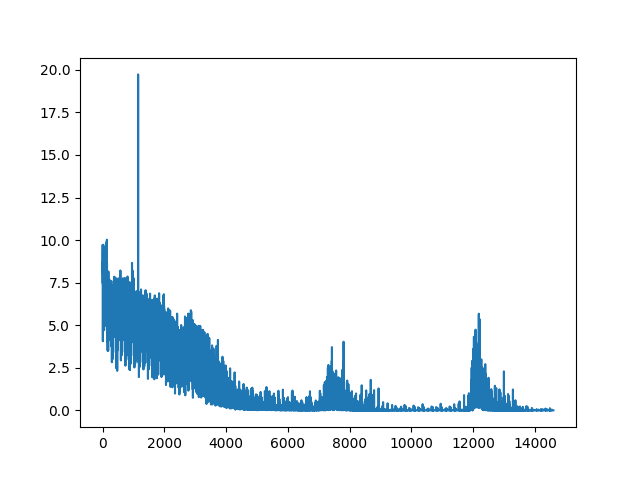
\includegraphics[scale=0.3]{images/slm_1e-3_101EP.png}
%		\caption{SLM-Model mit Lernrate 0.001 und Bahdanau's Additive Attention}
%		\label{SLM_lr1e-3}
%	\end{subfigure}
%	\hfill
%	\begin{subfigure}[b]{0.3\textwidth}
%		\centering
%		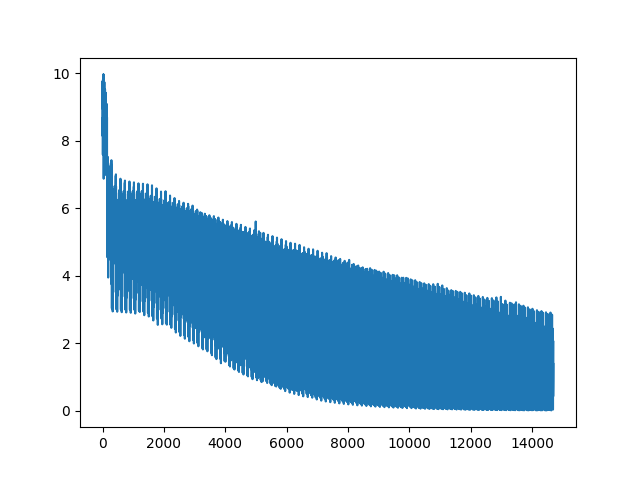
\includegraphics[scale=0.3]{images/bslm_bahdanau_2e_5_100EP.png}
%		\caption{BSLM-Model mit Lernrate 0.00002 und Bahdanau's Additive Attention}
%		\label{BSLM_Bahdanau_lr2e-5}
%	\end{subfigure}
%	\hfill
%	\begin{subfigure}[b]{0.3\textwidth}
%		\centering
%		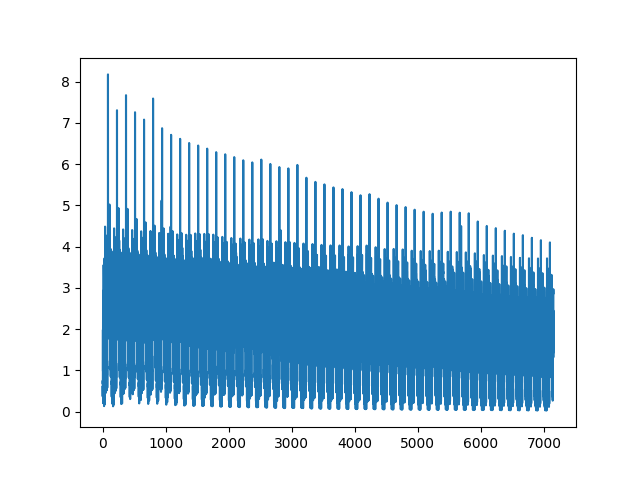
\includegraphics[scale=0.3]{images/bslm_luong_100EP_1e-5_PT3.png}
%		\caption{BSLM-Model mit Lernrate 0.00002 und Luongs's Multiplikative Attention}
%		\label{BSLM_Luong_lr2e-5}
%	\end{subfigure}
%	
%	\caption{Fehlerwerte der besten Modele nach BLEU-Score}
%	\label{fig:best_models}
%\end{figure}
%
%
%Aus den \cref{SLM_lr1e-3,BSLM_Bahdanau_lr2e-5,BSLM_Luong_lr2e-5} wird es deutlich, welches Model am besten lernt, das simple Model. An zweiter Stelle ordnet sich das BERT-Model mit Bahdanau Attention. Das beste BLEU-Score von den Luongs Modelen ist es, das für 150 Iterationen in 3 Phasen mit der Lernrate von 0.00001 lernt. Mit einem Score von unter 0.1 ist dieser Lernvorgehensweise nicht gerechtfertigt.
%
%Hier ist es wichtig zu erwähnen das die oben beschriebenen Tests (siehe \cref{SLM_lr1e-3,BSLM_Bahdanau_lr2e-5,BSLM_Luong_lr2e-5}) mehrfach ausgeführt wurden und die Ergebnisse waren jedes Mal die selben.
%
